\newpage
\section{Сетевое взаимодействие}
\setcounter{figure}{0}

Механизм TCP предоставляет поток данных с предварительной установкой соединения, осуществляет повторный запрос данных в случае потери данных и устраняет дублирование при получении двух копий одного пакета, гарантируя тем самым целостность передаваемых данных и уведомление отправителя о результатах передачи.

\subsection{Сетевое взамодействие в Qt Framework}

Сетевое взаимодействие в программах, написанных на языке C++ реализуется при помощи сокетов, в Qt для реализации данного взаимодействия используется надстройка над механизмом сокетов, облегчающая реализацию данного взаимодействия.

Данный механизм представлен такими классами как [3]:
\begin{itemize}
 \item QAbstrackSocket;
 \item QTcpSocket;
 \item QTcpServer;
 \item QUdpSocket.
\end{itemize}

Для реализации взаимодействия будут использоваться классы QTcpSocket и QTcpServer.

\subsection{УСПД}

Для тестирования программы реализован эмулятор, на базе одноплатного компьютера Raspberry Pi B+. Для этого компьютера был написан скрипт на языке python. Задачей скрипта является прослушивание порта и реакция на все приходящие команды их отправкой в обратном порядке. 

Текст скрипта:

\begin{lstlisting}
#!/usr/bin/python
# -*- coding: utf-8 -*-

import socket

sock = socket.socket()
sock.bind(('', 9090))
sock.listen(5)
while True:
        conn, addr = sock.accept()
        while True:
                data = conn.recv(1024)
                if not data:
                        break
                buf = data[::-1] + '\n'
                print data
                conn.send(buf)

conn.close()
\end{lstlisting}

\subsection{Взаимодействие с УСПД}

Для сетевого взаимодействия с УСПД была создана программа с графическим итерфейсом. Задачей данной программы является установление соединения с определенным адресом и получением/отправкой текстовой информации. Схема работы представлена на рисунке \ref{scheme1:scheme1}.

\begin{figure}[h!]
 \center{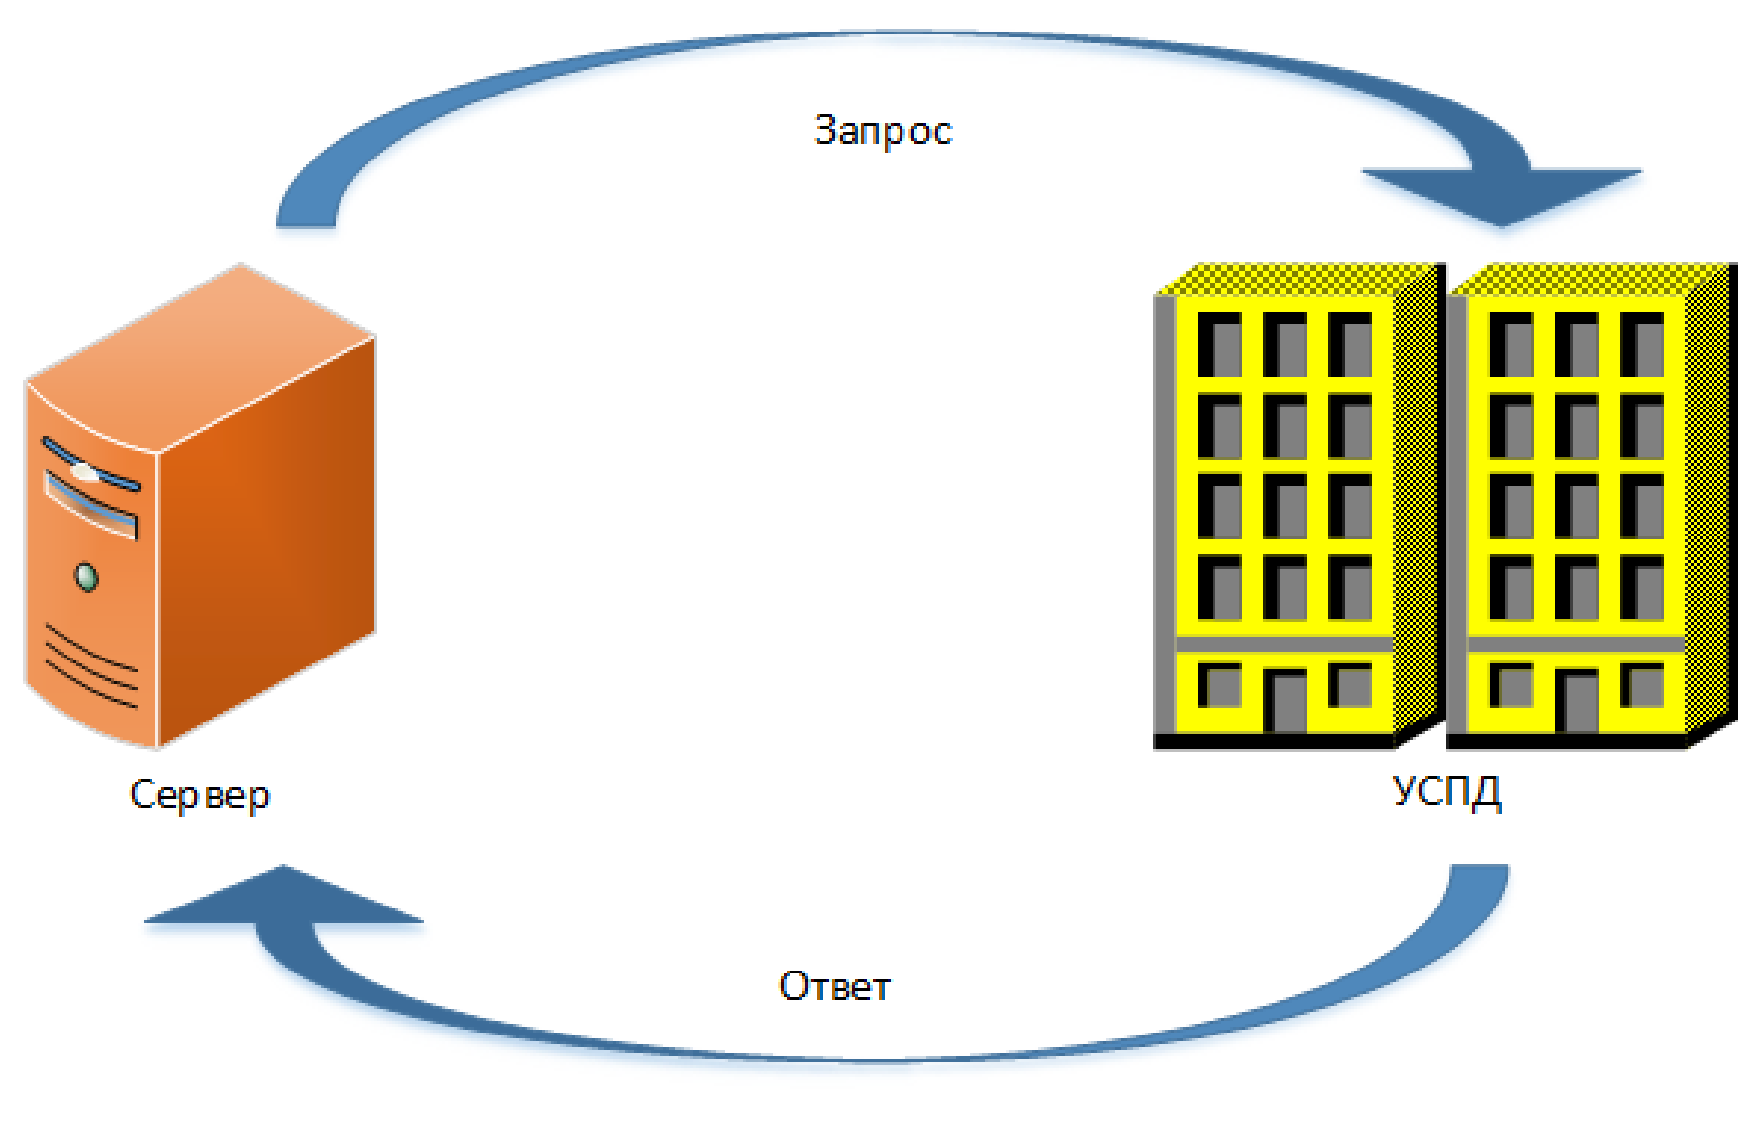
\includegraphics[width=0.8\linewidth]{scheme1}}
 \caption{Схема взаимодействия сервера с УСПД}
 \label{scheme1:scheme1}
\end{figure}

Прототип объекта, решающего эту задачу, выглядит так:

\begin{lstlisting}
class EmulSocket : public QObject
{
    Q_OBJECT
public:
    explicit EmulSocket(QObject *parent = 0);
    ~EmulSocket();
    void configure(QString, int);
    void initSocket();
    void sendData(QByteArray);

private:
    QString qs_Address;
    int i_Port;
    QTcpSocket * sc;
signals:
    void haveData(QString);
public slots:
    QString getData();
};
\end{lstlisting}

В конструкторе и диструкторе объекта инициализируется и уничтожается объект QTcpSocket *sc.

Метод configure(QString, int) заполняет значения ip-адреса и порта назначения (поля qs\_Address и i\_Port соответственно), так же в данном методе происходит связывание события ``приняты данные'' с обработчиком этого события - методом getData(). После чего вызывается метод initSocket().

Метод initSocket() отвечает за установление соединения с указанным хостом.

Метод sendData(QByteArray) - это функция, отправляющая полученный массив байт по адресу назначения.

Сигнал haveData(QString) - это вспомогательный сигнал для взаимодействия объекта с графическим интерфейсом.

Метод getData() обрабатывает входящий поток данный и при получении данных испускает сигнал haveData(QString) в котором передает полученные данные.

Интерфейс программы представлен на рисунке \ref{window1:window1}.

\begin{figure}[h!]
 \center{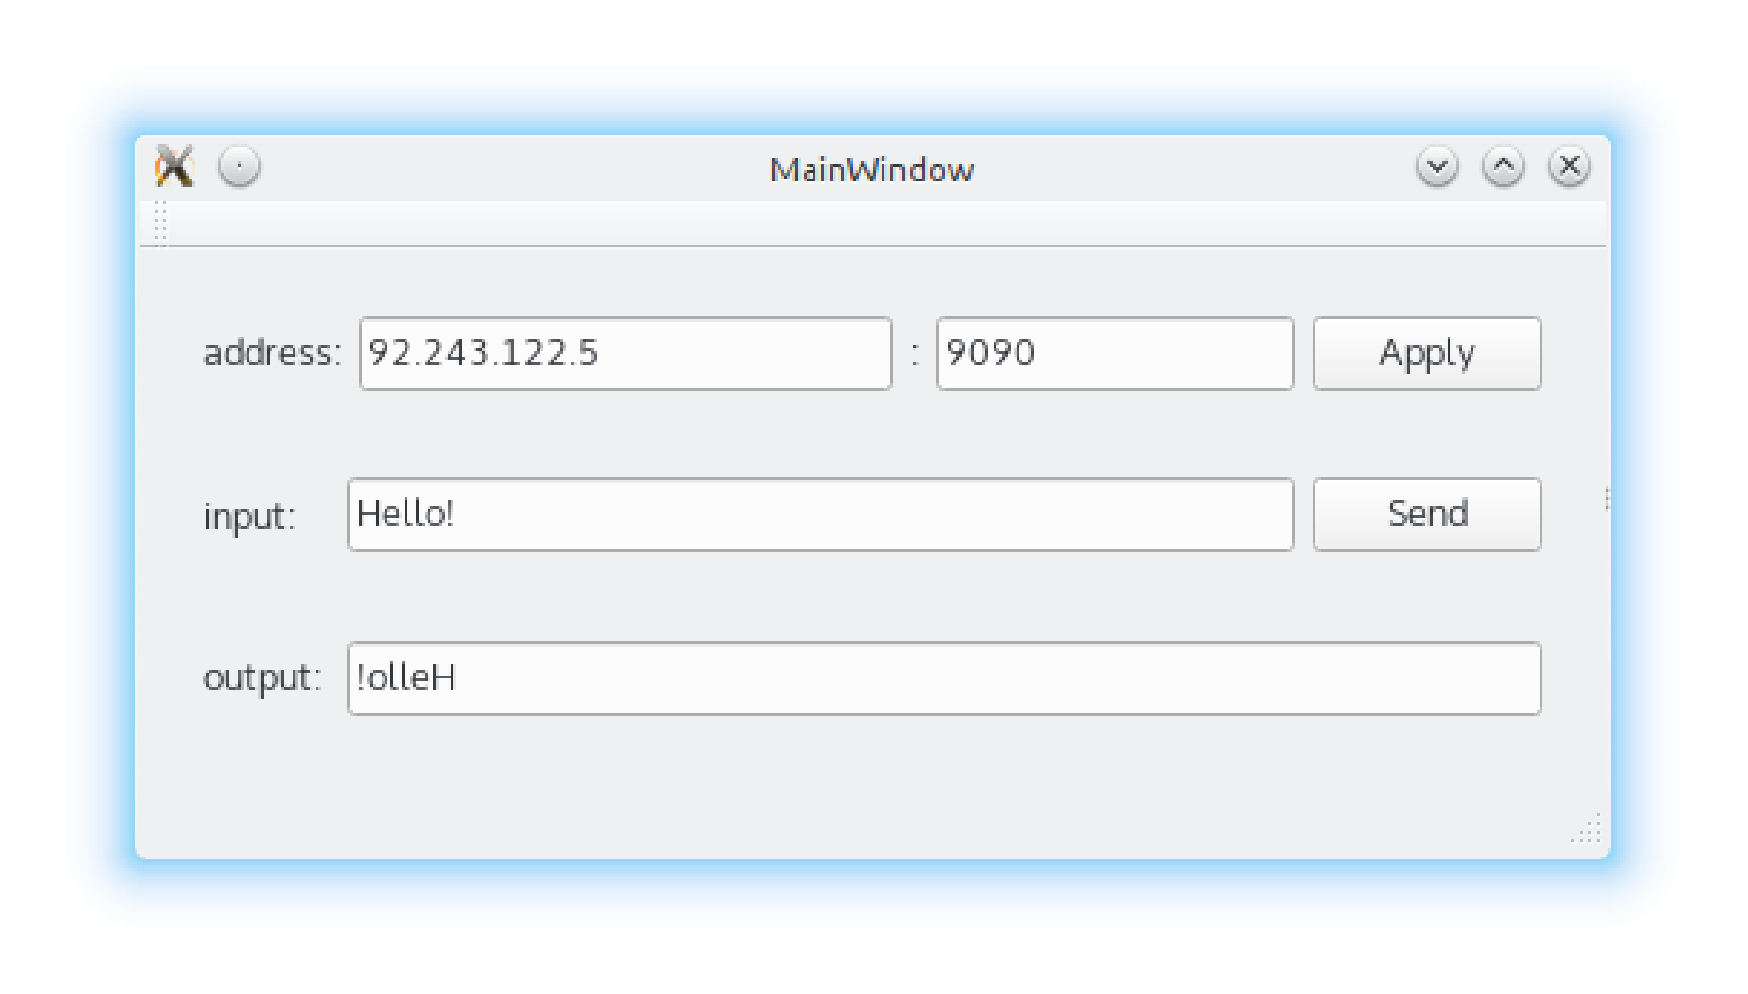
\includegraphics[width=0.7\linewidth]{window1}}
 \caption{Подключение к эмулятору УСПД}
 \label{window1:window1}
\end{figure}

Алгоритм работы программы представлен на рисунке \ref{alg1:alg1}.

\begin{figure}[h!]
 \center{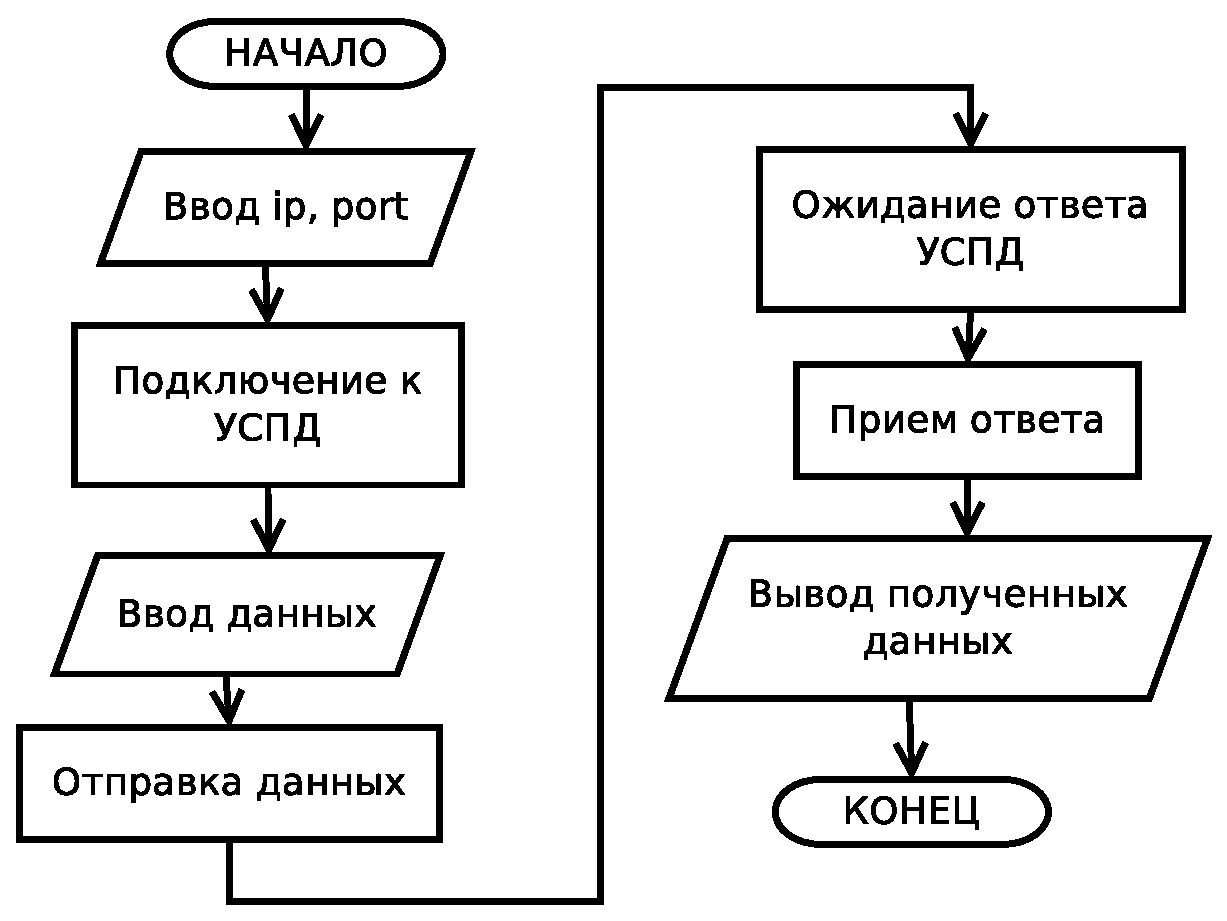
\includegraphics[width=0.8\linewidth]{alg1}}
 \caption{Алгоритм работы программы}
 \label{alg1:alg1}
\end{figure}


\subsection{Сохранение данных}

После установления связи с УСПД необходимо фиксировать полученную информацию в базе данных. Для теста была выбрана СУБД SQLite. 

В базу данных записываются ответы от УСПД с добавлением временной метки получения данных. Данные записываются в таблицу с тремя полями: id, data, time. Ниже представлен SQL-запрос создания описанной таблицы.

\begin{lstlisting}
 CREATE TABLE `list` (
	`id`	INTEGER PRIMARY KEY AUTOINCREMENT,
	`data`	TEXT NOT NULL,
	`time`	NUMERIC NOT NULL
	);
\end{lstlisting}


Для реализации данного функционала необходимо создать функции для работы с базой данных. Для этого в приложении (пункт 3.3) был добавлен новый объект. 

Описание объекта:

\begin{lstlisting}
class EmulDB : public QObject
{
    Q_OBJECT
public:
    explicit EmulDB(QObject *parent = 0);
    ~EmulDB();

    bool dbConnect(const QString& );
    void dbDisconnect();
    bool dbInsert(const QString& );

private:
    QSqlDatabase m_db;
    bool m_bOpen;
};
\end{lstlisting}

Конструктор и диструктор не выполняют каких либо дополнительных действий, атрибуты m\_db и m\_bOpen это база данных и её состояние (подключена ли база данных) соответственно.

Методы dbConnect и dbDisconnect необходимы для подключения и отключения к базе даных. 

Метод dbInsert принимает данные и записывает их в таблицу, подставляя время записи.

На рисунке \ref{dBase:dBase} представлено содержимое базы данных после тестового запуска программы.

\begin{figure}[h!]
 \center{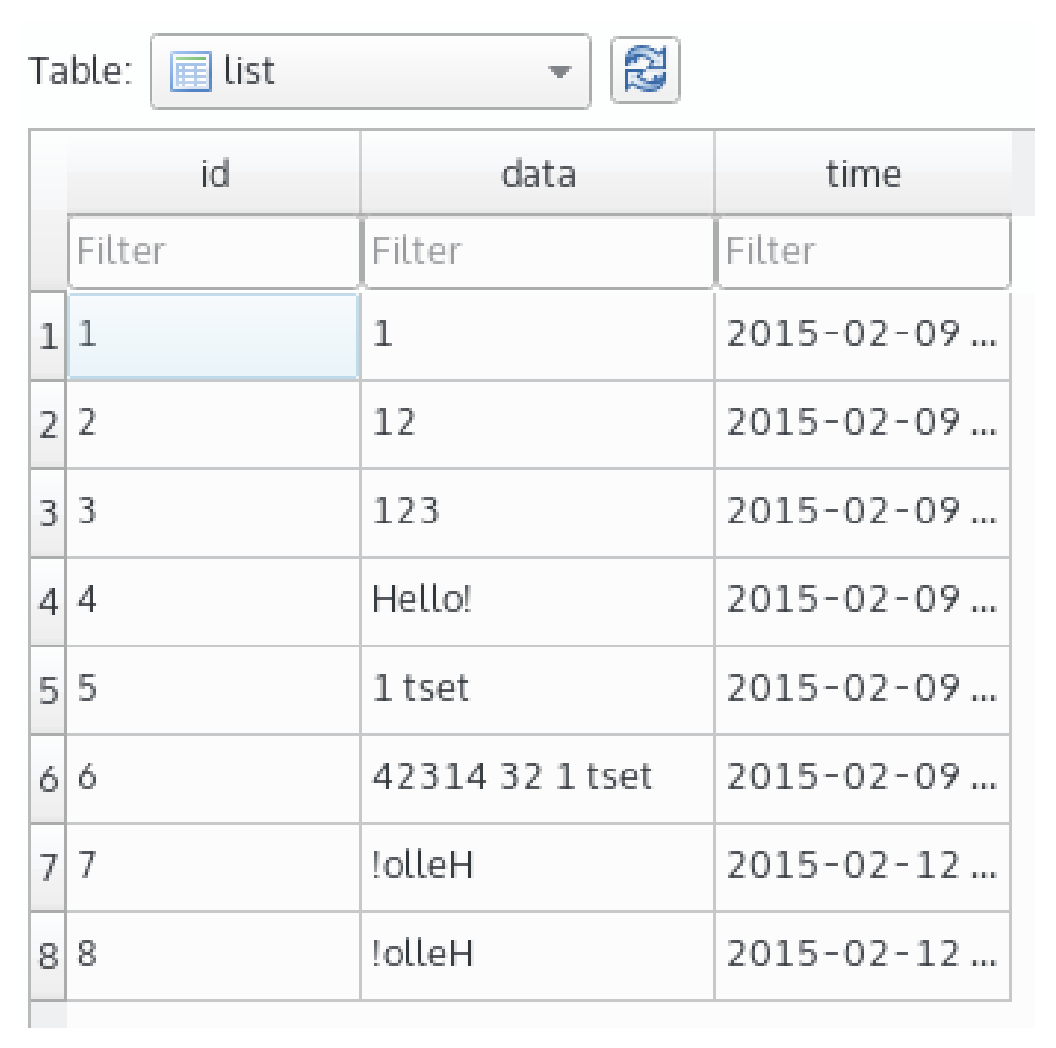
\includegraphics[width=0.7\linewidth]{dBase}}
 \caption{Просмотр таблицы}
 \label{dBase:dBase}
\end{figure}

Алгоритм работы программы представлен на рисунке \ref{alg2:alg2}.

\begin{figure}[h!]
 \center{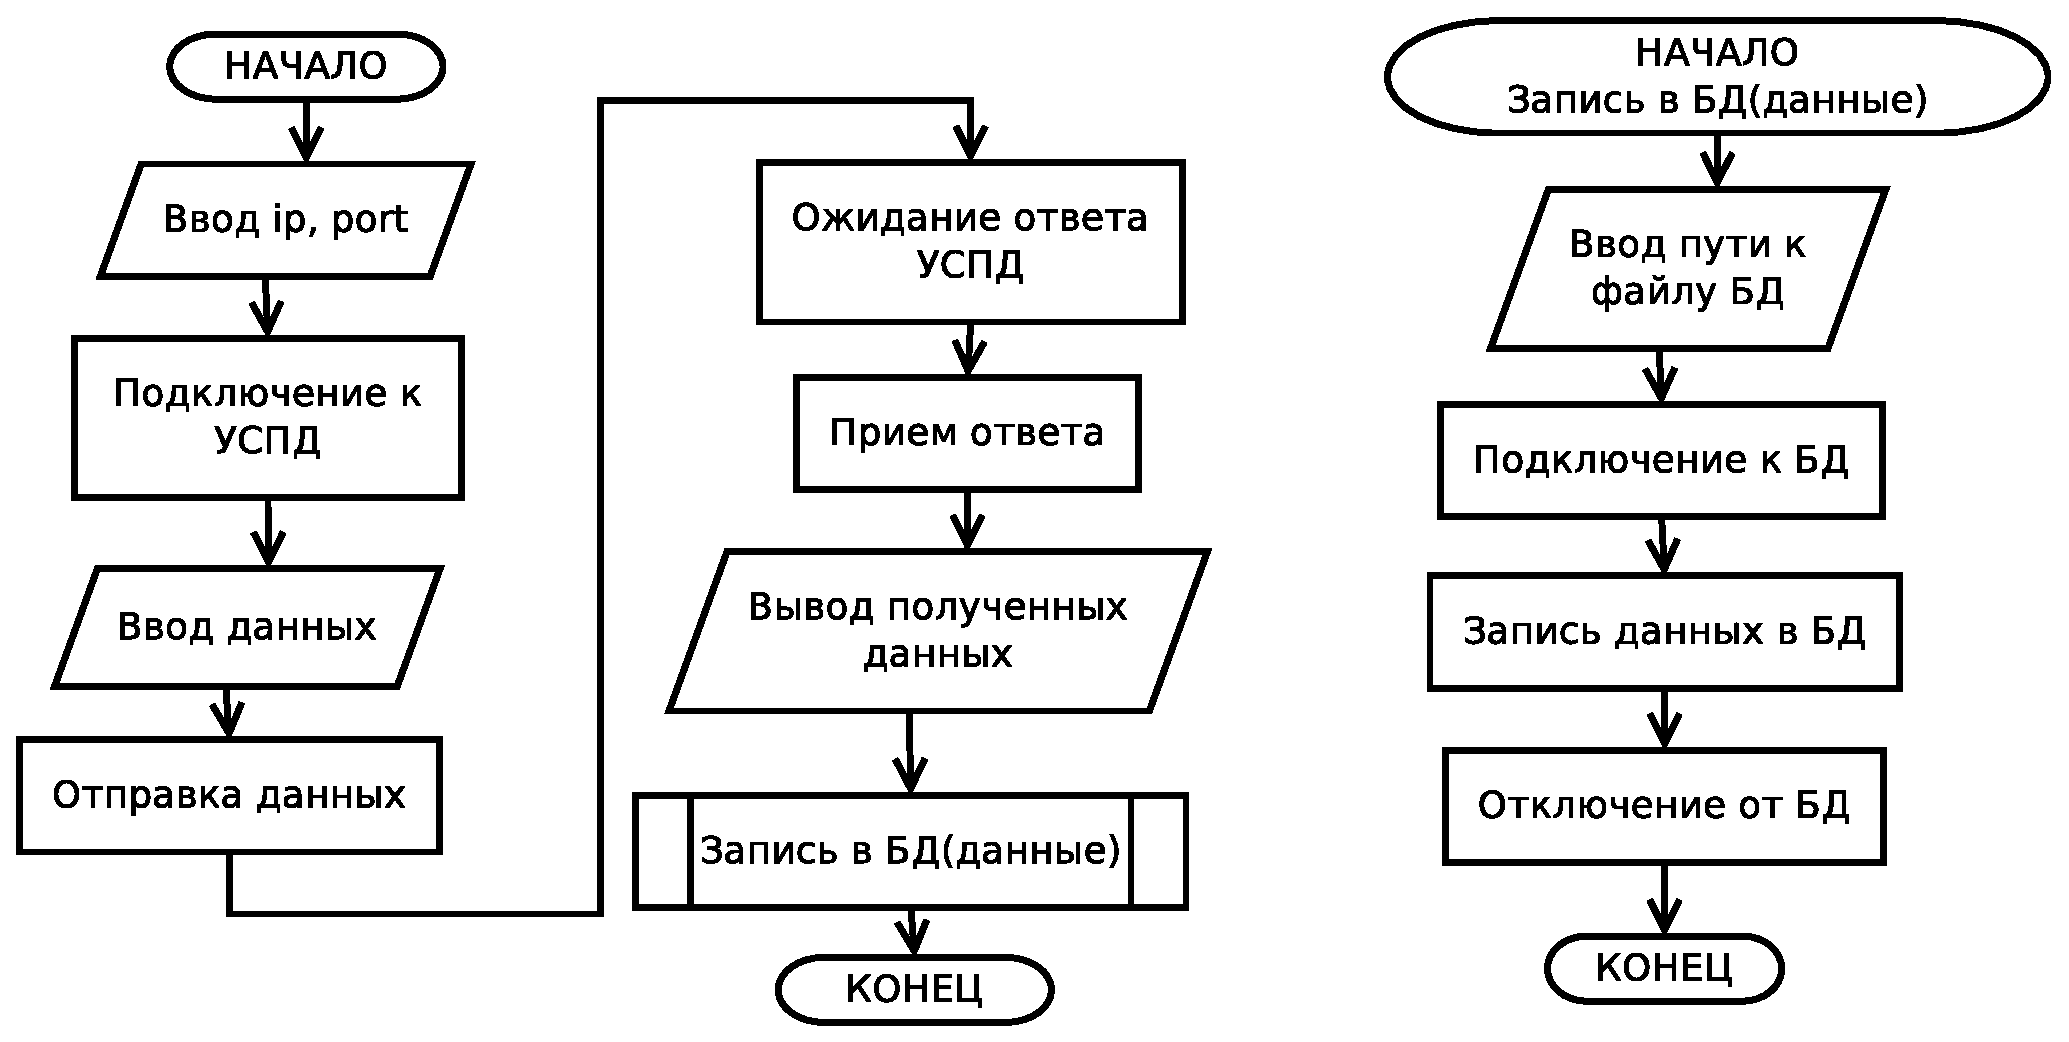
\includegraphics[width=0.8\linewidth]{alg2}}
 \caption{Алгоритм работы программы}
 \label{alg2:alg2}
\end{figure}